% !TeX root = ../thuthesis-example.tex

\chapter{VR-IOT RESEARCH PLATFORM PERFORMANCE TESTING}

The evaluation of creating devices and performing simultaneous work in the IoT-VR environment is an important part of this research. This chapter describes several experiments used for testing the NUIX-Studio platform performance.
There are several devices in the example configuration (Figure~\ref{fig:TestingEquipment-figure}):
\begin{enumerate}
    \item A Smart Wi-Fi lamp;
    \item A PC running openHAB server and NUIX-Studio App instance;
    \item A PC running NUIX-Studio App instance;
    \item An Oculus Quest VR Headset;
    \item A smart vacuum cleaner.
\end{enumerate}

\begin{figure}
  \centering
  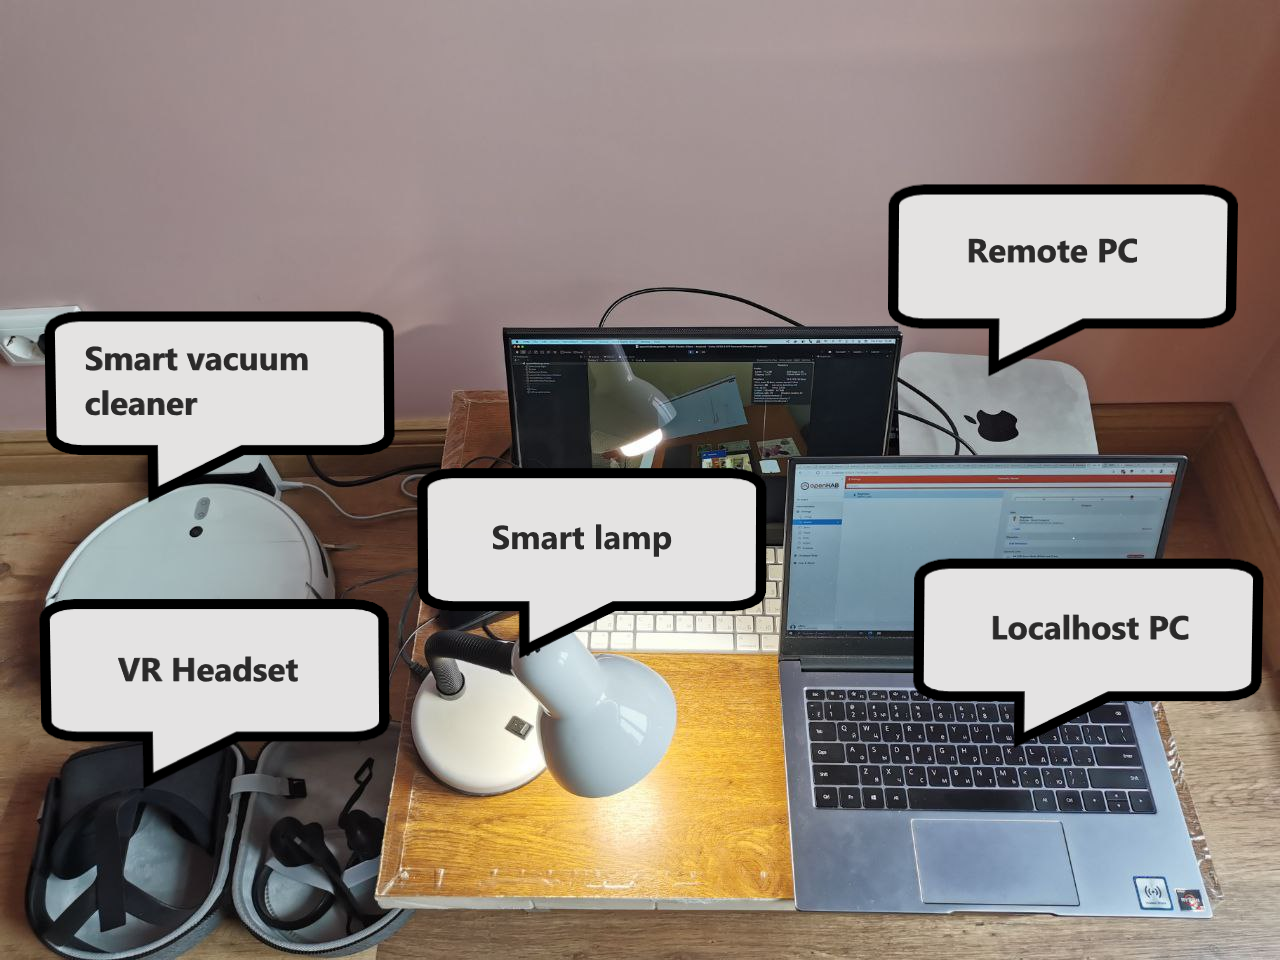
\includegraphics[width = 0.9 \linewidth]{figures/TestingEquipment.png}
  \caption{Testing equipment.}
  \label{fig:TestingEquipment-figure}
\end{figure}

In the first experiment, gesture control functionality is added for the smart lamp\footnote{Smart vacuum cleaner and remote PC will be used in the next experiments}. Widgets for Light and Gesture Recognition are created in the virtual environment scene. In other words, virtual lamp light is equivalent to the real-world one, and a gesture control interface is implemented.

\section{Server setup}
Same as in the previous chapter, Things representing the Smart Lamp and Vacuum Cleaner are added to the server by using a suitable Binding (Figure~\ref{fig:ServerSetupProcedure-figure}).

\begin{figure}
  \centering
  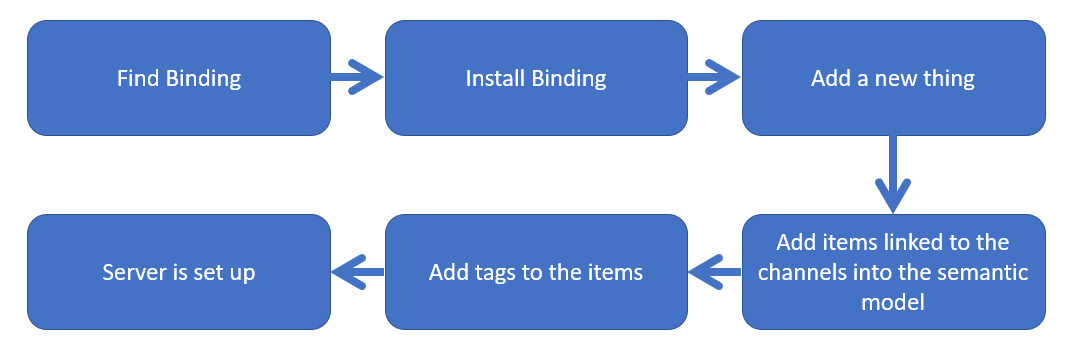
\includegraphics[width = 0.9 \linewidth]{figures/ServerSetupProcedure.png}
  \caption{Server setup procedure.}
  \label{fig:ServerSetupProcedure-figure}
\end{figure}

The next step is adding the Items linked to the Things' Channels. In the example, the lamp's brightness dimmer is added to the Semantic model. As seen in Figure~\ref{fig:SemanticModelOne-figure}, the user can move the dimmer to control the lamp's light brightness. The real-world lamp will change the brightness based on the value on the server.

\begin{figure}
  \centering
  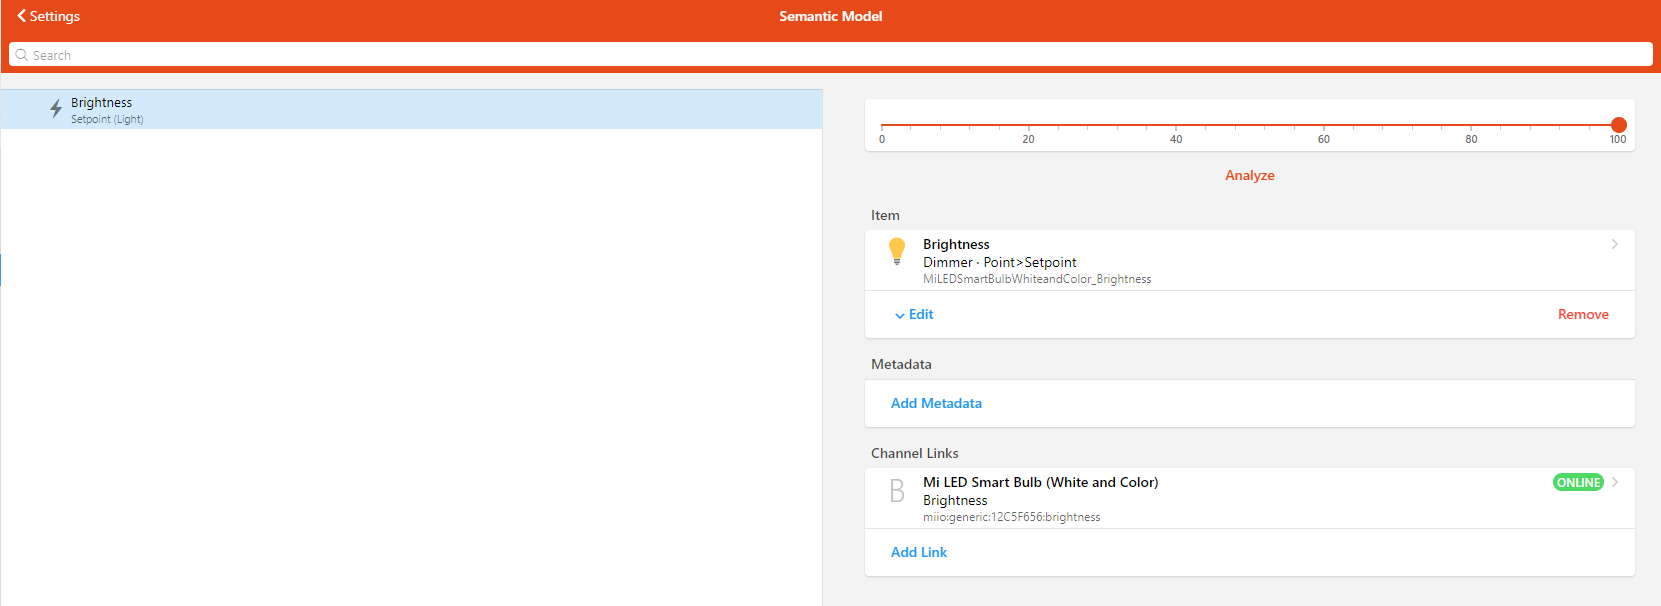
\includegraphics[width = 0.9 \linewidth]{figures/SemanticModelOne.png}
  \caption{The Semantic model in the first experiment}
  \label{fig:SemanticModelOne-figure}
\end{figure}

The next step is adding Item Tags for the Gesture and Brightness control (Figure~\ref{fig:ItemEditPage-figure}). Tags provide information for the NUIX-Studio App about which Widgets for the Item it needs to create.

\begin{figure}
  \centering
  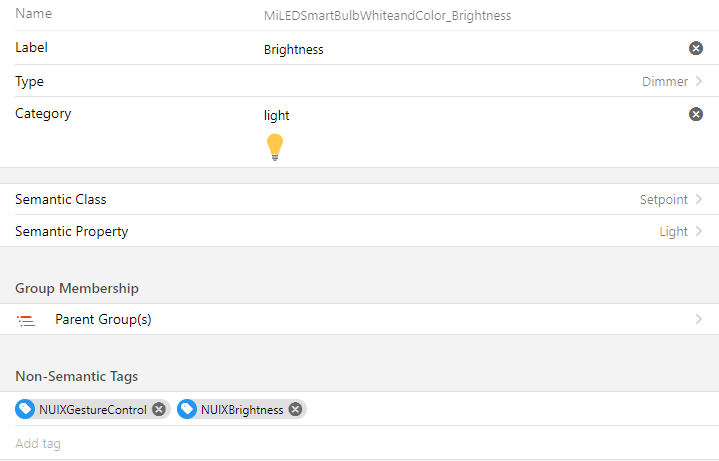
\includegraphics[width = 0.9 \linewidth]{figures/ItemEditPage.png}
  \caption{Item Edit Page.}
  \label{fig:ItemEditPage-figure}
\end{figure}

The server has been set up for connection to NUIX-Studio App instances.

\section{Running NUIX-Studio App}

In the experiment, a VR-IoT platform user performs three actions:
\begin{enumerate}
    \item Put on Virtual reality headset;
    \item Press the virtual button to establish a Client-Server connection and receive the items list;
    \item Perform a "Thumb up" gesture. By rotating the fist, the lamp brightness changes in the VR-IoT environment\footnote{Both in real and virtual worlds} (Figure~\ref{fig:FullBrightnessOculus-figure}).
\end{enumerate}


\begin{figure}
  \centering
  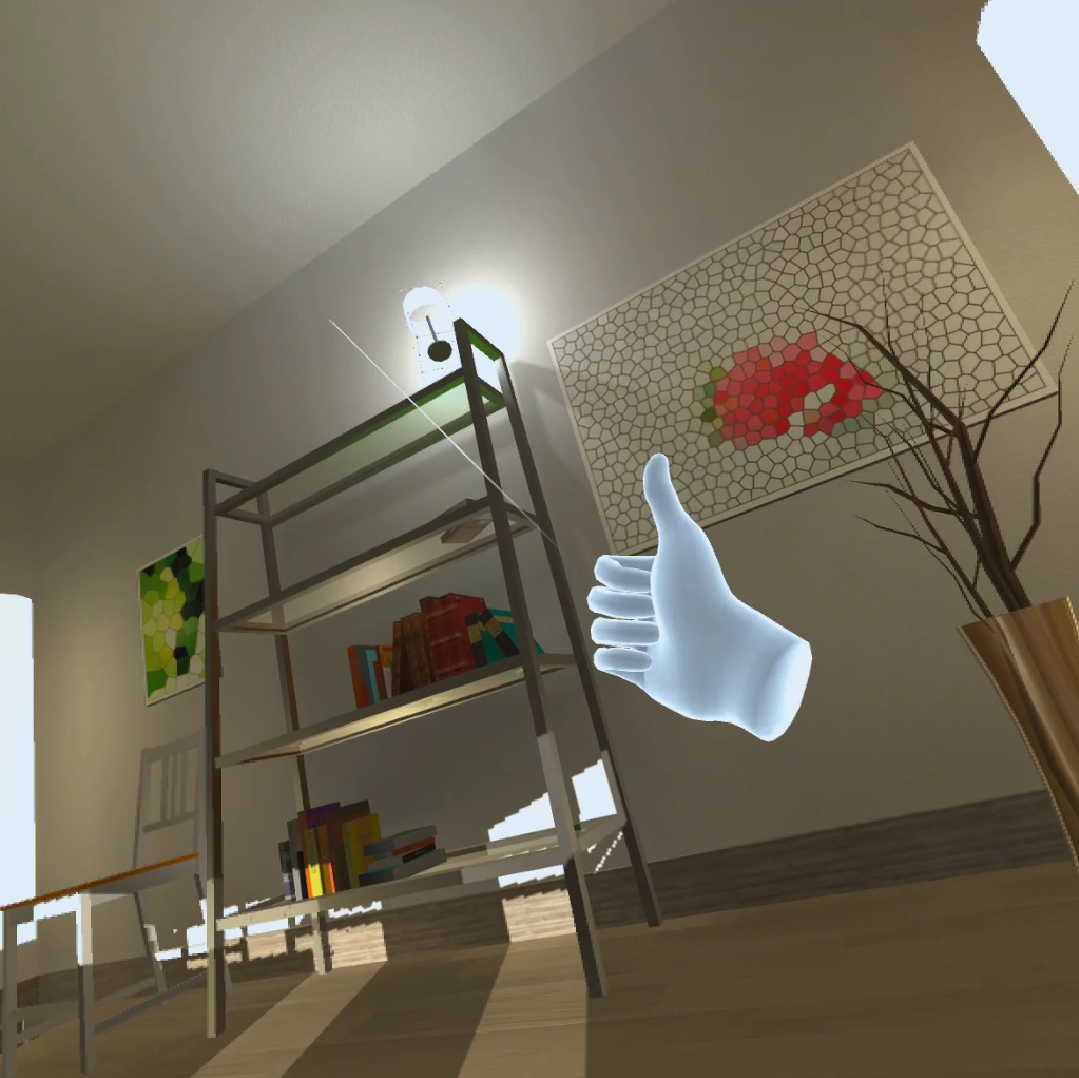
\includegraphics[width = 0.9 \linewidth]{figures/FullBrightnessOculus.png}
  \caption{"Thumb up" gesture.}
  \label{fig:FullBrightnessOculus-figure}
\end{figure}

The user of the platform performed these actions\footnote{In this experiment, the platform developer performed the user role.} (Figure~\ref{fig:BrightnessControl-figure}). Thus, support for gestures was added to control the lamp's brightness, and the experiment to create a new device for the existing environment can be considered a success.

\begin{figure}
  \centering
  \subcaptionbox{Lamp brightness set to ~75\%\label{fig:HalflBrightness}}
    {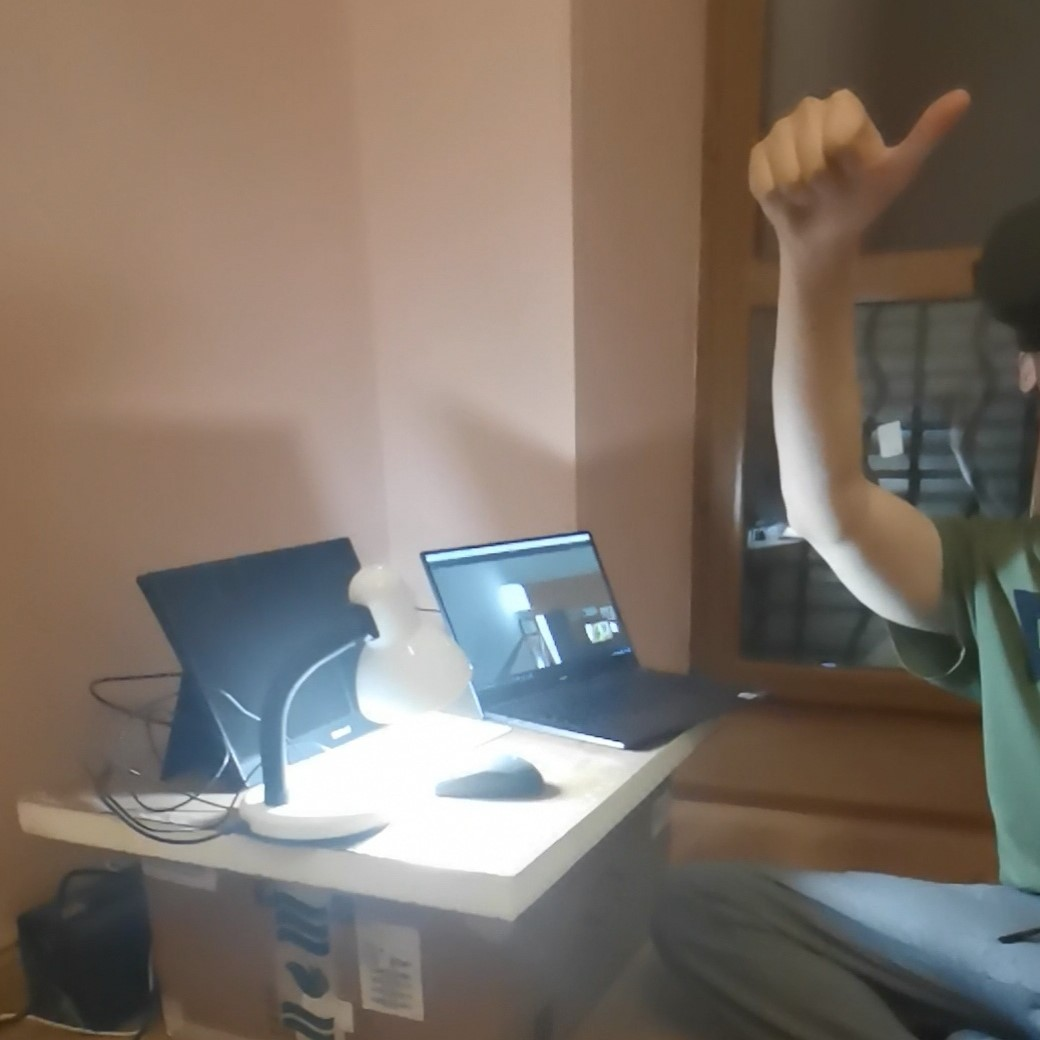
\includegraphics[width=0.45\linewidth]{figures/HalflBrightness.jpg}}
  \subcaptionbox{Lamp brightness set to 100\%\label{fig:FullBrightness}}
    {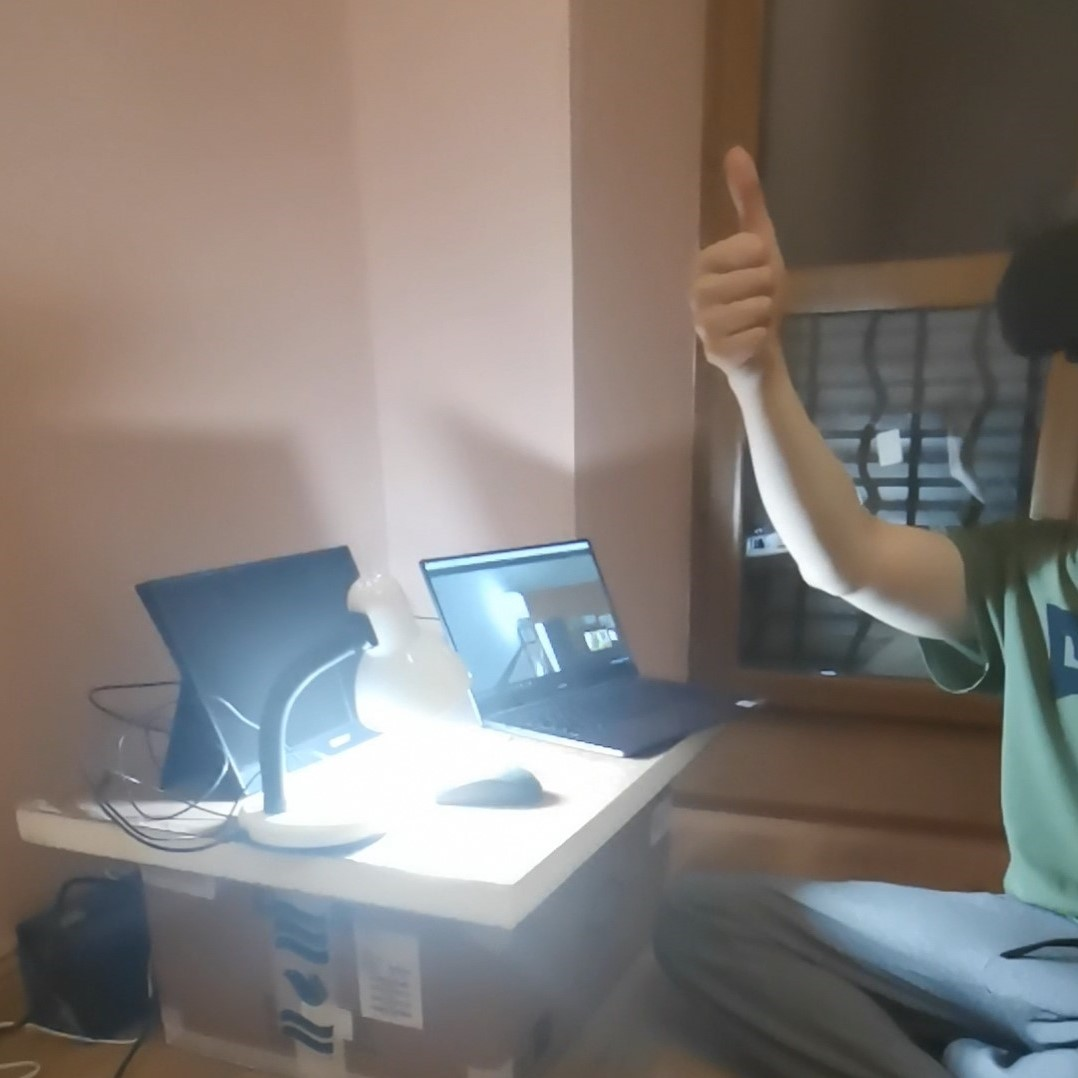
\includegraphics[width=0.45\linewidth]{figures/FullBrightness.jpg}}
  \caption{Experiment of the lamp brightness control. In both cases the real lamp and the NUIX-Studio App virtual lamps on Local PC and Oculus Quest brightness has the same value.}
  \label{fig:BrightnessControl-figure}
\end{figure}

\section{Performance analysis}

The analysis of platform performance is not the study's primary goal, but it helps to find bottlenecks. 

The following experiment shows that it is viable to perform rendering tasks on a separate server. Having a common database for all instances of the application will help achieve several users' simultaneous work within the system.

The first experiment is the system startup analysis, performed on three devices by registering the startup time (Figure~\ref{fig:SystemStartupScheme-figure}).

\begin{figure}
  \centering
  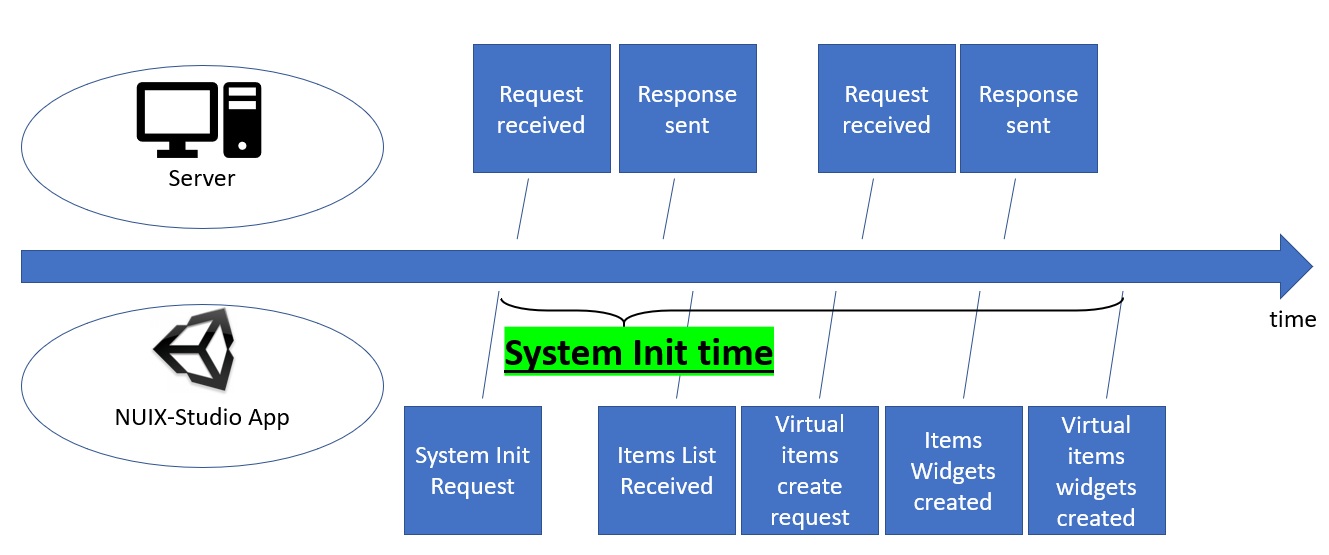
\includegraphics[width = 0.9 \linewidth]{figures/SystemStartupScheme.png}
  \caption{System startup scheme.}
  \label{fig:SystemStartupScheme-figure}
\end{figure}

The hardware specifications are listed in Table~\ref{tab:hardware-specifications-table} \footnote{Localhost PC is a notebook running openHAB server as well as one instance of NUIX-Studio APP; Remote PC is a computer running one instance of NUIX-Studio APP and connected to the same Wi-Fi network as localhost PC; Oculus Quest is a Virtual Reality Headset running NUIX-Studio APP and connected to the same Wi-Fi network as PCs.}.

\begin{table}
  \centering
  \begin{threeparttable}[c]
    \caption{Hardware specifications in the experimental setup}
    \label{tab:hardware-specifications-table}
    \begin{tabular}{ll}
      \toprule
      Unit    &         Specifications                 \\
      \midrule
      Localhost PC & Ryzen 5 3500u, Windows 10 \\
      Remote PC & Core i5 4278U, macOS 11.2.3    \\
      Oculus Quest        & Qualcomm Snapdragon 835, Android-based            \\
      \bottomrule
    \end{tabular}
  \end{threeparttable}
\end{table}

Each test was performed on a new Unity APP instance to avoid cashing influence. Then mean values for the tests have been calculated (Figure~\ref{fig:SystemInitTime-figure}).

\begin{figure}
  \centering
  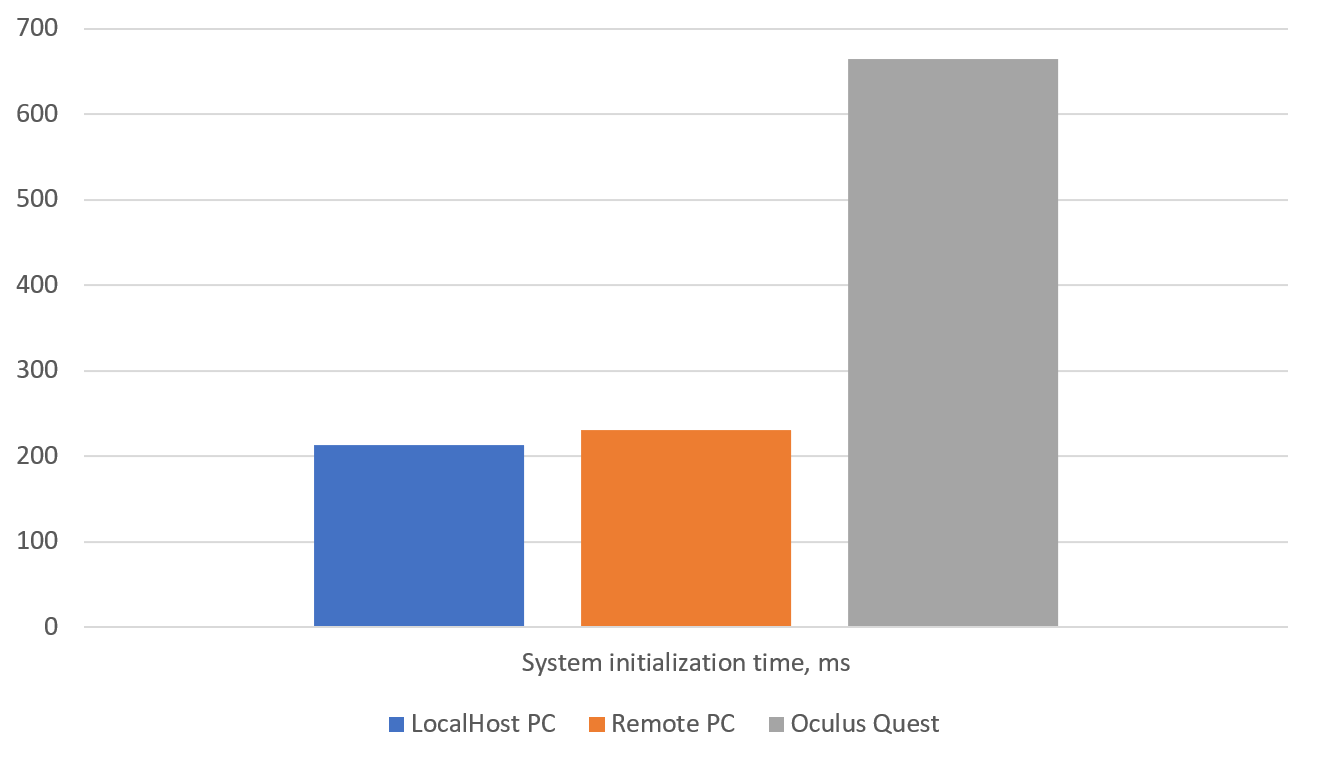
\includegraphics[width=0.9\linewidth]{figures/SystemInitTime.png}
  \caption{System initialization time measured on different client devices, in ms}
  \label{fig:SystemInitTime-figure}
\end{figure}

As seen in Figure~\ref{fig:SystemInitTime-figure}, the system initialization time is a time-consuming operation, which takes from 200ms to over 600ms on average to perform.

In the next experiment, event processing time was measured. On one of the devices running the NUIX-Studio App instance, a user changed an Item value \footnote{In this case, the brightness of the smart bulb changed by moving the corresponding pinch slider widget}. The server processed the received request to change the Item parameter, and then an Event containing information about the new Item value was sent to all devices connected to the server. The device on which this Item change occurred ignored the new incoming value because it was equal to the old value. Next, the processing time of a request on another device was measured (Figure~\ref{fig:EventProcessingScheme-figure}).

\begin{figure}
  \centering
  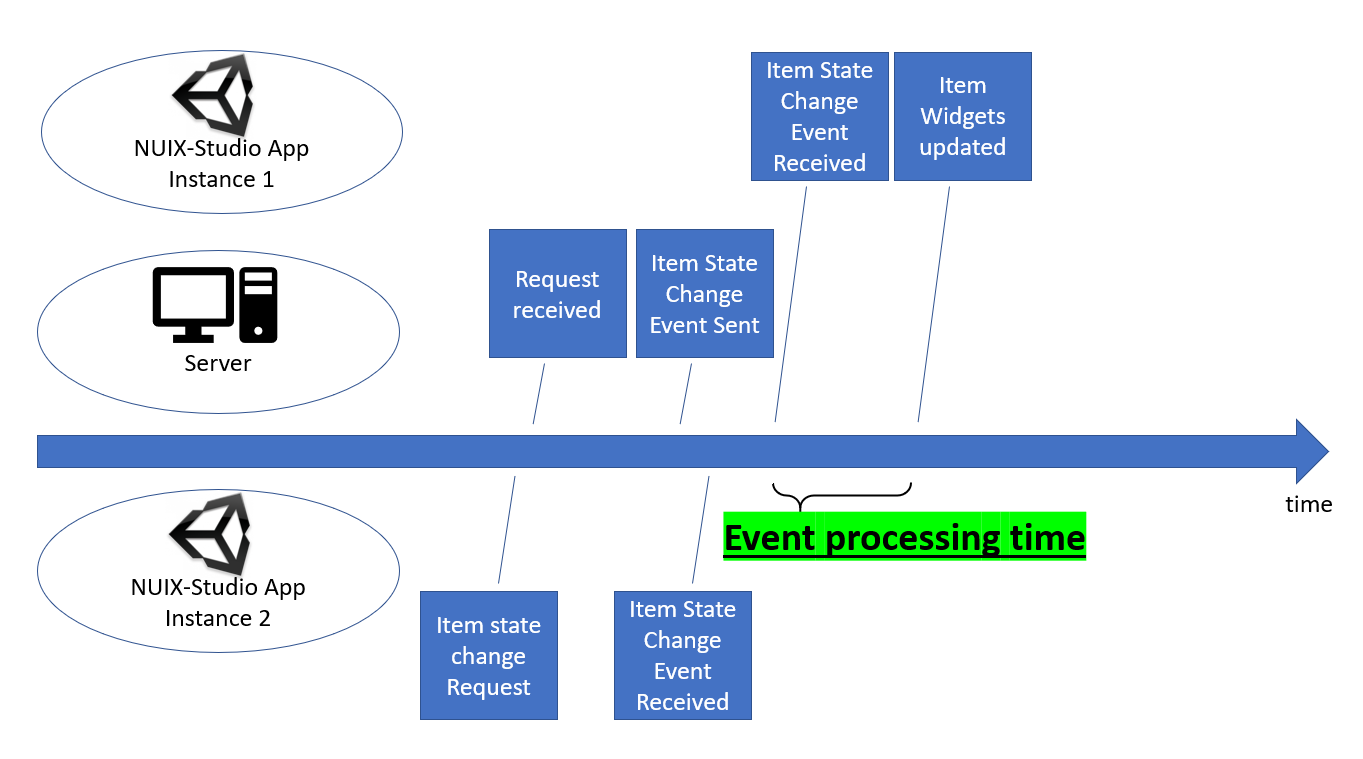
\includegraphics[width = 0.9 \linewidth]{figures/EventProcessingScheme.png}
  \caption{Event processing scheme.}
  \label{fig:EventProcessingScheme-figure}
\end{figure}

As seen on the resulting histogram (Figure~\ref{fig:EventProcessingTime-figure}), Oculus Quest's performance on this test is outstanding. The processing time difference is explained by the fact that the NUIX-Studio App runs in an unoptimized state on Windows and macOS\footnote{Unity editor mode}, but can run significantly faster after the App instances are built for the platforms.

\begin{figure}
  \centering
  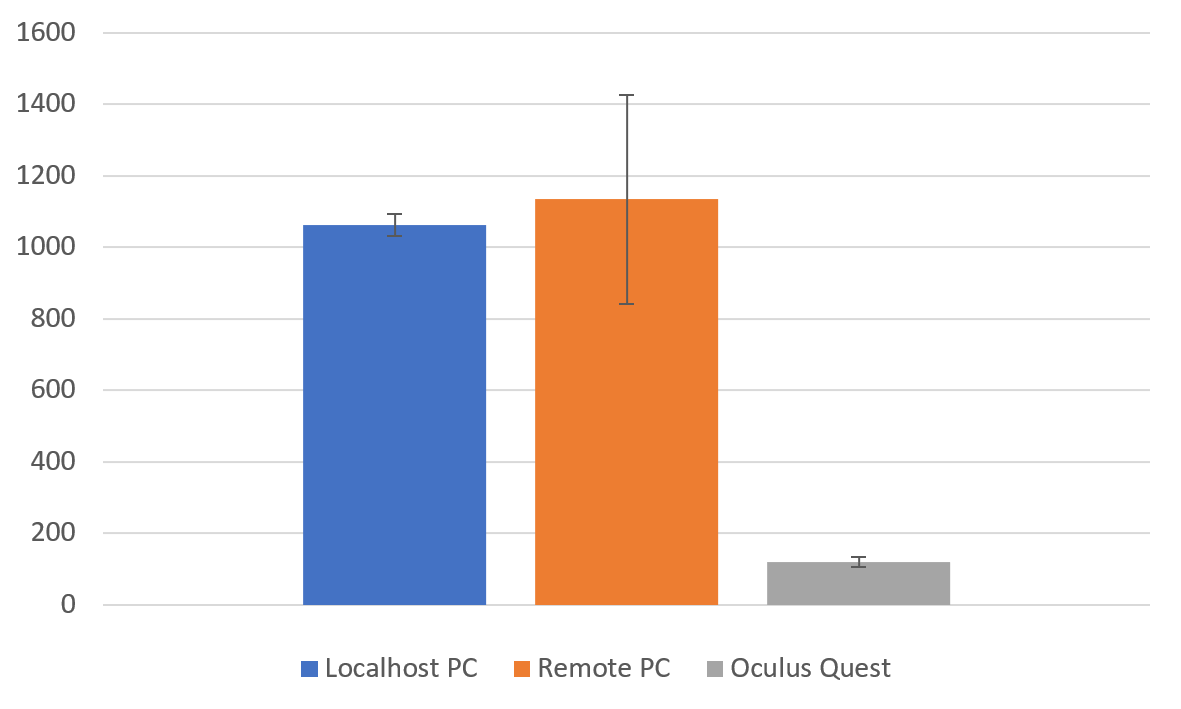
\includegraphics[width = 0.9 \linewidth]{figures/EventProcessingTime.png}
  \caption{Event processing time measured on different devices, in \textmu{}s}
  \label{fig:EventProcessingTime-figure}
\end{figure}

The results of this experiment will be used in the future: system initialization time is based on the device hardware performance, and in some later experiments, it is better not to perform time calculations that include system initialization, while event processing time is relatively low for each device, and in most cases, it can be ignored.

The following experiment uses a Virtual reality headset, a smart light bulb, and a server running an application on it. For instance, a light sensor is used inside a Smart home environment, located at a relatively large distance from the lamp (2-3 meters), and is triggered when the amount of light falling on its sensor exceeds a certain threshold. For example, this setup is used in industries to provide a comfortable lighting level while keeping an optimal amount of energy consumption. The light sensor triggers precisely at some sufficiently large value of the lamp brightness. Hence, the most accurate adjustment of the brightness level of the light bulb is needed.

The previous experiment showed that gesture control could be used to control a lamp's brightness level. This experiment shows that the transfer of computations from the Virtual reality headset to the server is necessary for specific scenarios. The user is asked to perform the same steps as in the previous experiment, with one more step added:  setting the brightness to the specified level. Supposing that the light sensor is triggered at a lamp light brightness level of 50 out of 100 \footnote{Using Fitts' law, it can be assumed that setting up brightness levels to different values takes different time. However, this effect is considered not significant for the experiment.}. The user's task is to set the light brightness to the specified value as quickly as possible using gesture control. In order to omit additional operations not related to the direct use of gestures to change the brightness of the lamp, such as starting the system, the user had to repeat the step by setting the brightness of the light to the specified value twiice. The interval between the first and second times, when the lamp brightness is equal to the specified value, can be divided into two components (Equation \eqref{eq:totaltime}): the user reaction time to a successful change in the brightness level $ t_{react} $, and the execution time of the new calibrations $ t_{cal} $.


\begin{equation}
  t = t_{react} + t_{cal}
  \label{eq:totaltime}
\end{equation}

Two people participated in the two series of the experiment. In the first series, the light's illumination was computed on a Virtual reality headset, and in the second, on a server that was periodically calculating the light map. User reaction time $ t_{react} $ is a value independent of the changed synchronization parameters. Therefore, the difference in calculated time in the first and the second series of the experiment is equal to the difference in time spent on calibrating the lamp brightness in the said experiment (Equation \eqref{eq:deltatime}).

\begin{equation}
  t _{\Delta} = (t_{react} + t_{cal_1}) - (t_{react} + t_{cal_1}) = t_{cal_1} - t_{cal_2}
  \label{eq:deltatime}
\end{equation}

As it can be seen in the Figure~\ref{fig:ExperimentTime-figure}, the time it took the participants to perform the task is unstable, but it is still can be seen that on average, it took more time to perform the task in the first series than in the second series for both users. In Figure~\ref{fig:DeltaTime-figure} it can be seen that $t_{\Delta}$ is more than zero for the most observations.

\begin{figure}
  \centering
  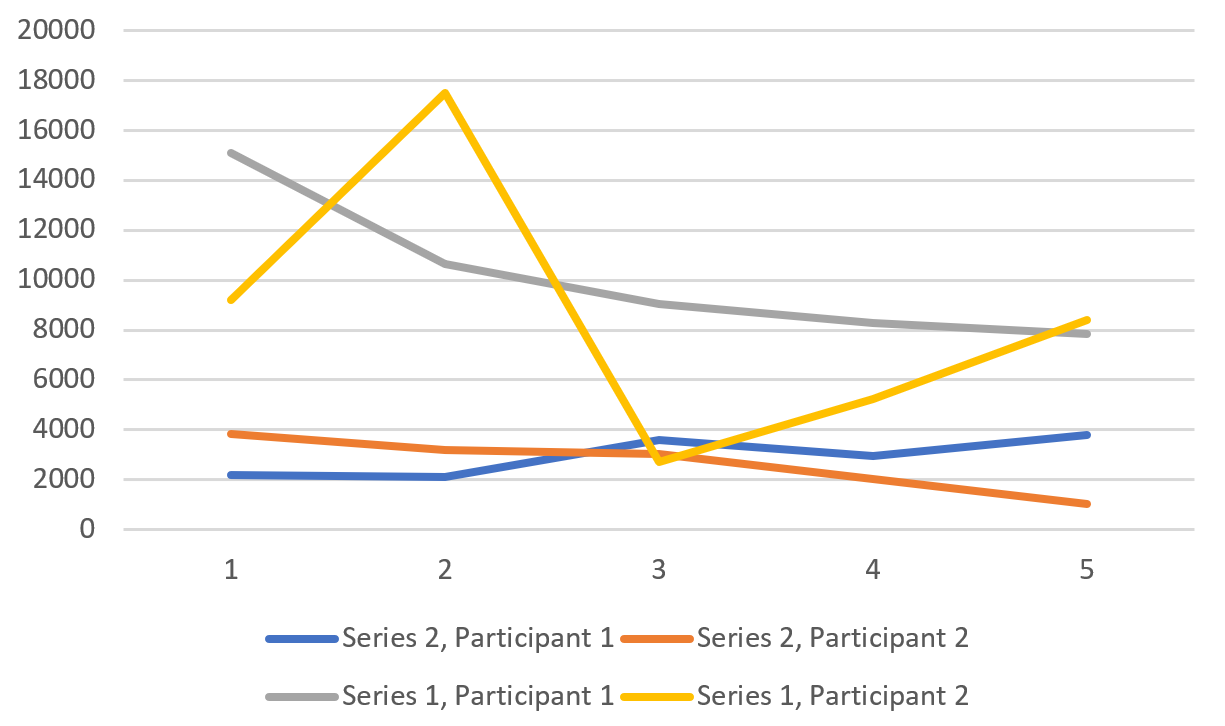
\includegraphics[width = 0.9 \linewidth]{figures/ExperimentTime.png}
  \caption{Time spent on calibrating the lamp brightness, in ms}
  \label{fig:ExperimentTime-figure}
\end{figure}


\begin{figure}
  \centering
  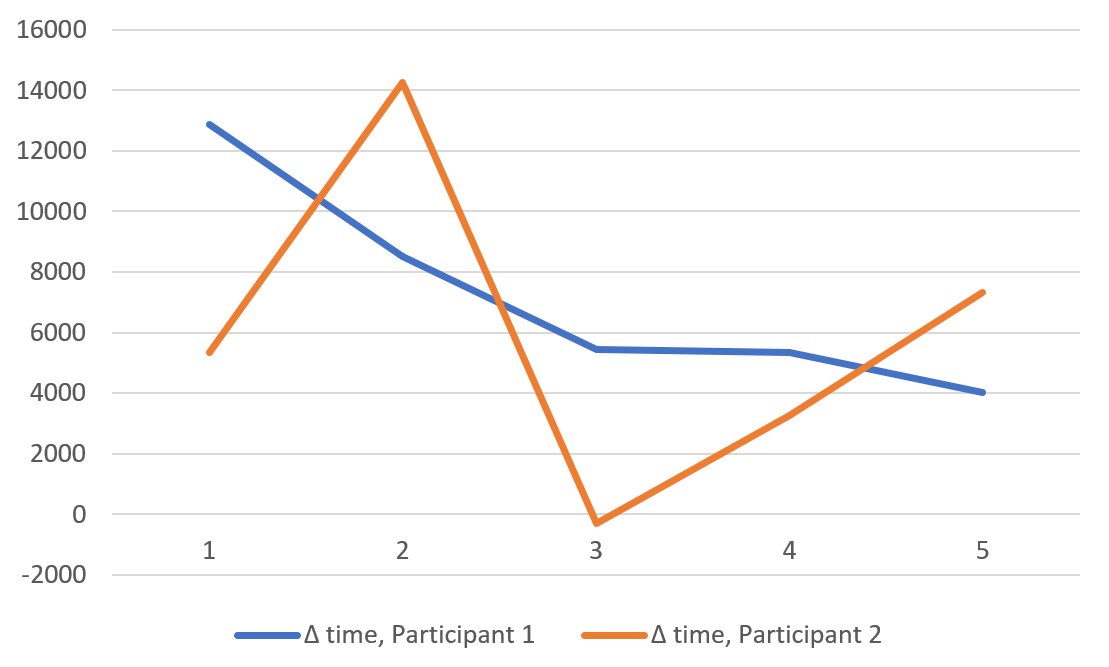
\includegraphics[width = 0.9 \linewidth]{figures/DeltaTime.png}
  \caption{The difference between the time spent on calibrating the lamp brightness in the first and the second series of the experiment, in ms}
  \label{fig:DeltaTime-figure}
\end{figure}

Additional data were analyzed during the experiment, such as the number of frames per second with which the NUIX-Studio App was rendered on the screen (Figure~\ref{fig:exp-screenshot}). Figure~\ref{fig:Series2FPSpng-figure} shows that in the first series of the experiment, the number of frames per second drops significantly as soon as the system is initialized and widgets for items from the Semantic model are created. In the second series of the experiment, such a drop is no longer observed (Figure~\ref{fig:Series1FPSpng-figure}): because the illumination was computed on a separate device, the number of frames per second drops only slightly \footnote{Probably, because illumination computation is significant for the device's performance, especially its Graphics processing unit.}.

\begin{figure}
  \centering
  \subcaptionbox{Series 1\label{fig:exp-screenshot-a}}
    {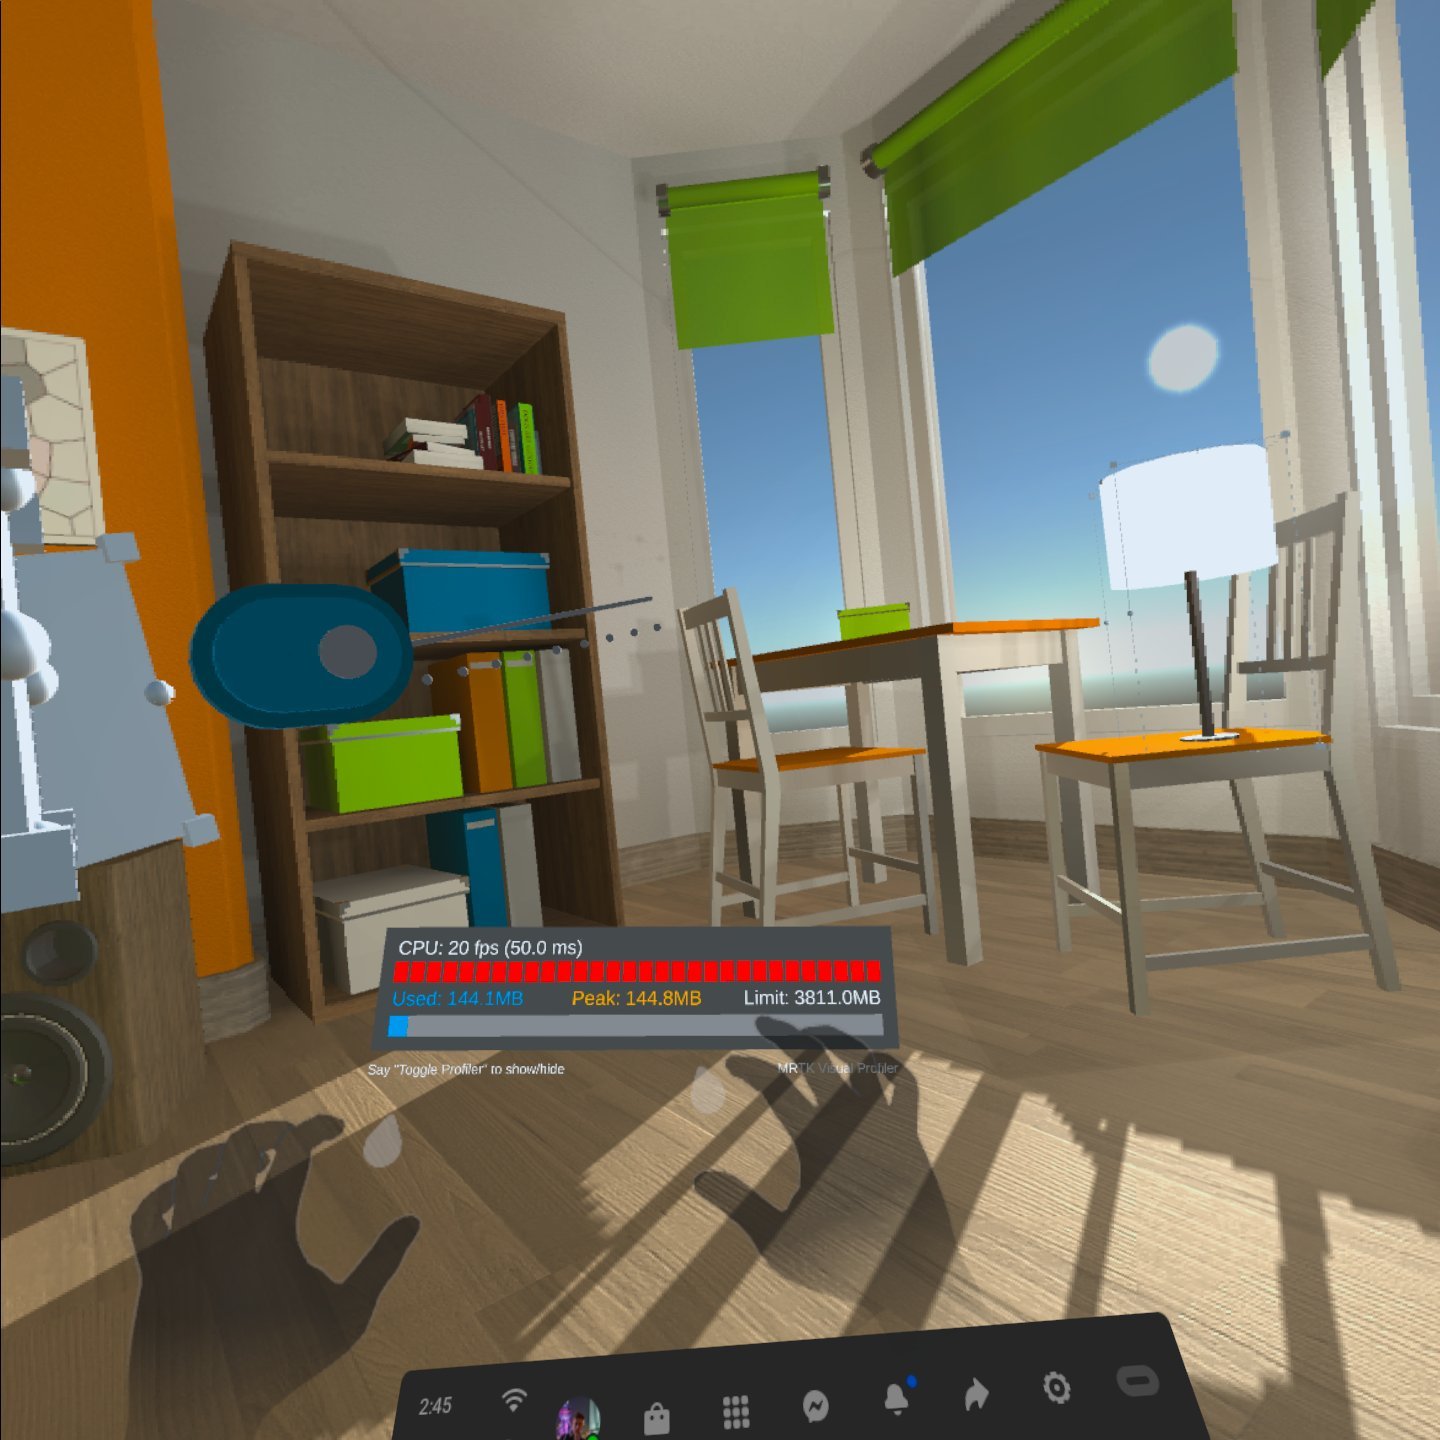
\includegraphics[width=0.45\linewidth]{figures/Series1FPSOculus.jpg}}
  \subcaptionbox{Series 2\label{fig:exp-screenshot-b}}
    {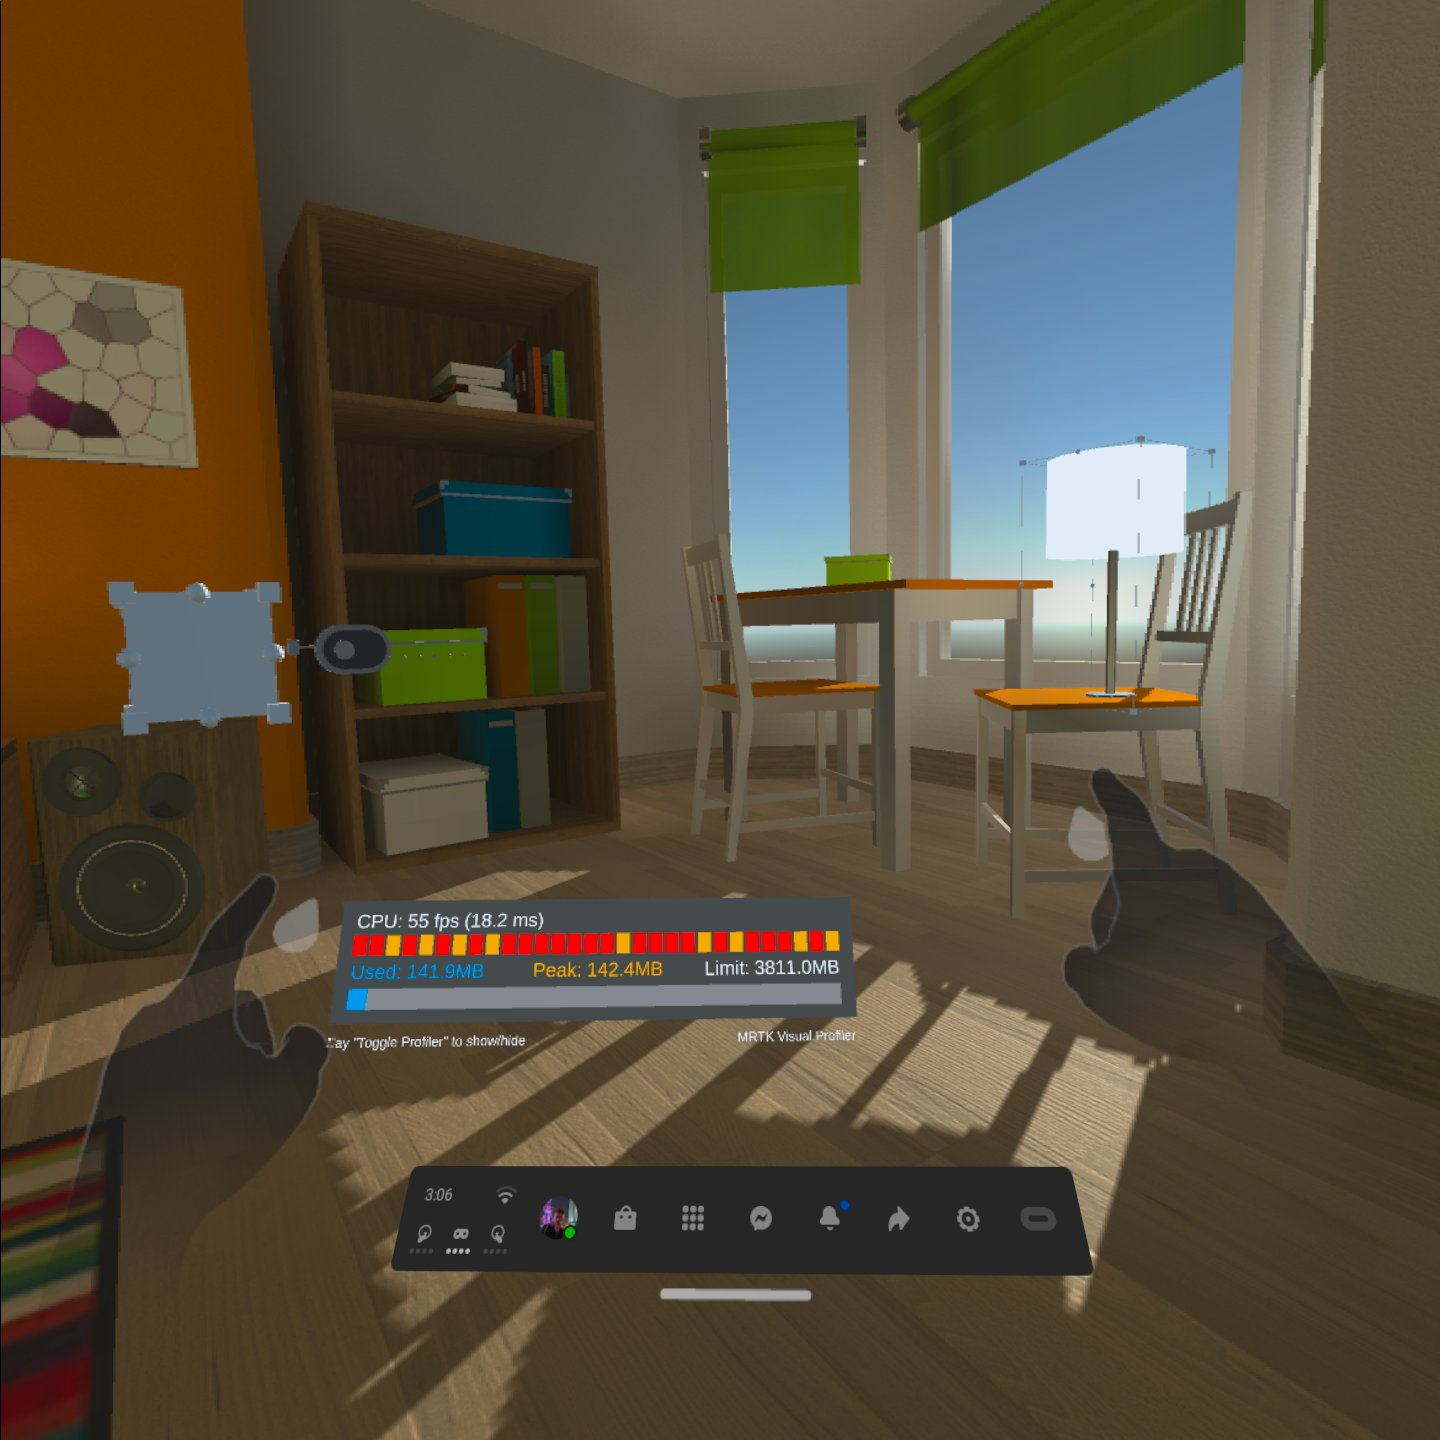
\includegraphics[width=0.45\linewidth]{figures/Series2FPSOculus.jpg}}
  \caption{Screenshots of the experiment.}
  \label{fig:exp-screenshot}
\end{figure}

\begin{figure}
  \centering
  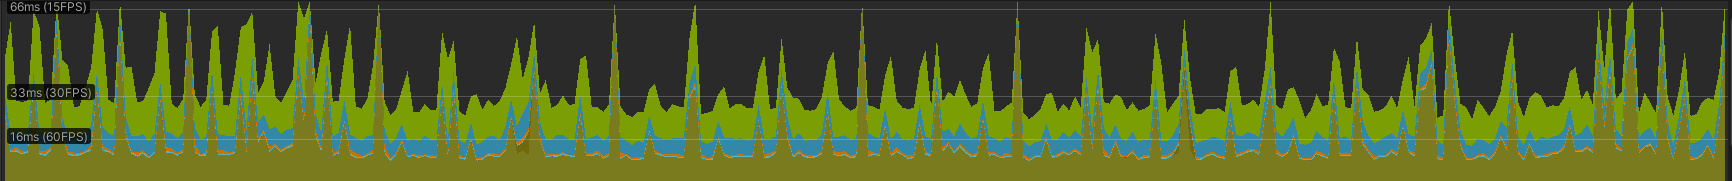
\includegraphics[width = 0.9 \linewidth]{figures/Series2FPSpng.png}
  \caption{FPS graph during the first series of the experiment of computations transfer.}
  \label{fig:Series2FPSpng-figure}
\end{figure}

\begin{figure}
  \centering
  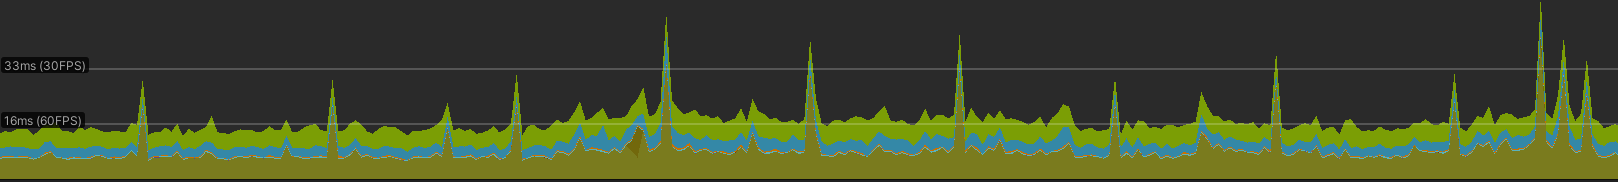
\includegraphics[width = 0.9 \linewidth]{figures/Series1FPS.png}
  \caption{FPS graph during the second series of the experiment of computations transfer.}
  \label{fig:Series1FPSpng-figure}
\end{figure}

Considering that gesture recognition is processed no more than once per frame, it significantly influenced the user experience, resulting in a big $t_{\Delta}$. The frequency of gesture value retrieval can be called polling rate. When a polling rate is 1000Hz, the gesture position is retrieved once every millisecond(Table~\ref{tab:polling-rate-table}). Probably, there is a linear dependency between the time spent on performing the calibration and the polling rate during the test.

\begin{table}
  \centering
  \begin{threeparttable}[c]
    \caption{Polling rate to response time of gesture recognition dependence}
    \label{tab:polling-rate-table}
    \begin{tabular}{ll}
      \toprule
      Polling rate, Hz    & Response time, ms                 \\
      \midrule
      72Hz & 13.9ms \\
      65Hz & 15.4ms \\
      20Hz & 50ms \\
      10Hz & 100ms \\
      \bottomrule
    \end{tabular}
  \end{threeparttable}
\end{table}

However, the experiment's main challenge was to show how transferring resource-intensive computing from a VR headset to a server improves user experience, significant for the VR-IoT Research platform. Thus, the experiment can be considered successful.\footnote{Please note that this experiment cannot be considered scientifically substantiated since the number of tests and the number of participants is relatively small. In addition, it is impossible to control the external factors that add random error, such as system optimization that affects the stability of the frame rate, room lighting that affects the accuracy of hand recognition, the size of the participants' hands, and the participants' experience with virtual reality systems. As a result, the reproduction of this experiment is almost impossible. Nevertheless, this experiment serves as an example of the requirement to transfer resource-intensive computing from the VR headset to the server.
}


In the next experiment, the author proved that it is possible to work together in one VR-IoT environment by adding new IoT devices to the system and changing their parameters:
\begin{enumerate}
    \item The time for adding a device to the system is limited by the performance of a specific platform and the speed of the Internet connection within the Wi-Fi network. When running 300 sequential ping tests from remote PC to localhost PC, all the values ​​obtained were less than 100ms, with 90 percent values ​​ranging from 45ms to 70ms. The time spent by the device on creating widgets for a smart vacuum cleaner roughly corresponded to the time of system initialization;
    \item Time interval from changing an Item on the remote PC to updating the widgets on localhost PC did not exceed 60ms.
\end{enumerate}

Thus, the speed of the network plays a significant role in the operation of the system. The minimal network latency available now in Wi-Fi 6 networks and 6G networks in the future can significantly improve the simultaneous work inside the same VR-IoT environment. However, it has been observed that operations such as adding new devices to the system will remain time-consuming. Since there is a request to create game objects for each of the Item's widgets, the author assumes that the main delay is associated precisely with the internal processes inside the Unity 3D engine.

The next chapter shows how the VR-IoT research platform developers can theoretically work around these limitations.